\chapter{Central force motions}
It was Newton's fascination with planetary motion that led him to formulate his laws of motion and the law of universal gravitation. His success in explaining Kepler's empirical laws of planetary motion was an overwhelming argument in favor of the new mechanics and marked the beginning of modern mathematical physics. Planetary motion and the more general problem of motion under a central force continue to play an important role in most branches of physics and turn up in such topics as particle scattering, atomic structure, and space navigation.
\section{Central force}
A central force  acting on a particle only depends upon magnitude of a distance from a fixed center. If $r$ is the instanteneous position vector of the particle relative to the fixed center. Then the central force is represented by the relation,
\begin{equation}
F= f(r) \hat{r}
\end{equation}
Where, $f(r)$ is a scalar function of distance, $r$  and $\hat{r}=\frac{\vec{r}}{r}$. Then the torque acting on the particle is,
\begin{equation}
\tau =r\times F
\end{equation}
This type of motion is particularly relevant when studying the orbital movement of planets and satellites. The laws which govern this motion were first postulated by Kepler and deduced from observation. In this lecture, we will see that these laws are a consequence of Newton's second law. An understanding of central force motion is necessary for the design of satellites and space vehicles.
\subsection{General Properties of Central Force Motion}
\begin{enumerate}
	
	\item The central force $f(r) \hat{{r}}$ is along ${r}$ and can exert no torque on the reduced mass $\mu $ , therefore angular momentum about centre of force is conserved. This implies that central force motion is a planar motion. 
	\begin{align*}
	\tau &=r\times F\\
	&=r  \hat{r} \times f(r) \hat{{r}}\\
	&=0 \quad (\text{Since,  } \hat{r} \times \hat{r} =0)
	\end{align*}
	\item Central forces are conservative, therefore total energy of a particle moving under central force is conserved.
	\item The magnitude of the angular momentum $|{L}| \equiv l$, and the total energy $E $ , of central force motion is constant.
	\item Areal velocity is constant, that is area swept by line joining the particle to the centre of force per unit time is constant.
	\begin{equation}
	\frac{\Delta A}{\Delta t}=\text { constant }
	\end{equation}
\end{enumerate}
\section{The two body central force problems}
\subsection{Reduction of two-body problems to one body problem}
A two-body system can be effectively reduced to one-body system by introducing the concept of reduced mass. Suppose a system is composed of two masses $m_{1}$ and $m_{2}$, then for an inertial observer the relative motion of these masses may be expressed by a fictitious particle of reduced mass $\mu$.\\
Let the instantaneous position of masses $m_{1}$ and $m_{2}$ be represented by position vectors $r_{1}$ and $r_{2}$ relative to an arbitrary origin 0\\
\begin{figure}[H]
	\centering
	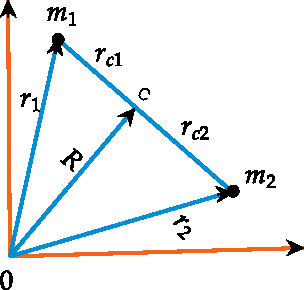
\includegraphics[height=5cm,width=5cm]{diagram-20220217(5)-20220217171814-crop}
	\caption{}
	\label{}
\end{figure}
Let us assume that no external force acts on the system and the internal force is simply due to mutual interaction of the particles, so the potential energy function is dependent only on internal forces, so the potential energy function may be assumed to be the function of vector between two particles $\mathbf{r}_{2}-\mathbf{r}_{1}$ or their relative velocity $\left(\dot{\mathbf{r}}_{2}-\dot{\mathbf{r}}_{1}\right) .$ This system has six degrees of freedom and hence requires six independent generalised coordinates. We choose these to be three components of radius vector $\mathbf{R}$ of centre of mass and three components of difference vector $\mathbf{r}=\mathbf{r}_{2}-\mathbf{r}_{1}$.\\
The Lagrangian of the system has the form $L=T(\dot{\mathbf{R}}, \dot{\mathbf{r}})-V(\mathbf{r}, \dot{\mathbf{r}}, \ldots)$
The kinetic energy of the system may be expressed as the sum of kinetic energy of the motion of centre of mass plus the kinetic energy of the motion about the centre of mass, i.e.,
$$
T=\frac{1}{2}\left(m_{1}+m_{2}\right) \dot{\mathbf{R}}^{2}+\left(\frac{1}{2} m_{1} \cdot{\mathbf{r}}_{C_{1}}^{2}+\frac{1}{2} m_{2} \cdot{\mathbf{r}}_{C_{2}}^{2}\right)
$$
where $\mathbf{r}_{C_{1}}$ and $\mathbf{r}_{C_{2}}$ are the radii vectors of the two particles relative to centre of mass. $\mathbf{r}_{C_{1}}$ and $\mathbf{r}_{C_{2}}$ are related to $\mathbf{r}$ by the equations\\
$$\left.\begin{array}{l}
	\mathbf{r}_{C_{1}}=-\frac{m_{2}}{m_{1}+m_{2}} \mathbf{r} \\
	\mathbf{r}_{C_{2}}=\frac{m_{1}}{m_{1}+m_{2}} \mathbf{r}
\end{array}\right\}$$
Substituting these values, we get
$$
T=\frac{1}{2}\left(m_{1}+m_{2}\right) \dot{\mathbf{R}}^{2}+\frac{1}{2}\left(\frac{m_{1} m_{2}}{m_{1}+m_{2}}\right) \dot{\mathbf{r}}^{2}
$$
so the Lagrangian of the system
$$
L=T-V=\frac{1}{2}\left(m_{1}+m_{2}\right) \dot{\mathbf{R}}^{2}+\frac{1}{2}\left(\frac{m_{1} m_{2}}{m_{1}+m_{2}}\right) \dot{\mathbf{r}}^{2}-V(\mathbf{r}, \dot{\mathbf{r}})
$$
$\mathbf{R}$ does not occurs in Lagrangian, so three components of $\mathbf{R}$ are cyclic, so centre of mass is either at rest or in uniform motion. No equation of motion for $\mathbf{r}$, will contain terms containing $\mathbf{R}$ or $\dot{\mathbf{R}}$, so assuming centre of mass at rest, me may drop the first term from the Lagrangian, i.e.,
$$
L=\frac{1}{2}\left(\frac{m_{1} m_{2}}{m_{1}+m_{2}}\right) \dot{\mathbf{r}}^{2}-V(\mathbf{r}, \dot{\mathbf{r}}, \ldots)
$$
$\text { This is the Lagrangian of a single particle of a fictitious mass } \mu=\frac{m_{1} m_{2}}{m_{1}+m_{2}} \text { placed at the }$ at the location of $m_2$ with the original potential function.Thus two body problem is equivalent to one body problem.
\subsection{The equation of motion and first integral}
Let us consider only the central force, where the potential $V$ is the function of $r$ only, so that the force is always directed along $\mathbf{r}$. Let a single particle move about a fixed centre of force which we assume to be the origin of co-ordinate system. Using polar co-ordinates $(r, \theta)$, the kinetic energy of particle is given by\\
$T=\frac{1}{2} \mu\left(\dot{r}^{2}+r^{2} \dot{\theta}^{2}\right), \mu$ being reduced mass.\\
The potential energy $V=V(r)$.\\
The Lagrangian of the system is given by

\begin{align}
&L=T-V \\
&=\frac{1}{2} \mu\left(\dot{r}^{2}+r^{2} \dot{\theta}^{2}\right)-V(r) .\\
\intertext { Lagrange's equation for } \theta \text { is } &\frac{d}{d t}\left(\frac{\partial L}{\partial \dot{\theta}}\right)-\frac{\partial L}{\partial \theta}=0
\end{align}
$\therefore \quad$ From (2.5)
$$
\frac{\partial L}{\partial \theta}=0 \text { and } \frac{\partial L}{\partial \dot{\theta}}=\mu r^{2} \dot{\theta}
$$
$\therefore \quad$ From (2.6)
$$
\frac{d}{d t}\left(\mu r^{2} \dot{\theta}\right)=0
$$
Integrating, we get\\
\begin{align}
\mu r^{2} \dot{\theta}= constant =J (say),
\end{align}
where $J$ is first integral (constant of motion) and represents the magnitude of angular momentum.\\
As $\mu$ is constant, equation (2.6) gives\\
\begin{align}
	&\frac{d}{d t}\left(r^{2} \dot{\theta}\right)=0 \notag\\
	&\frac{d}{d t}\left(\frac{1}{2} r^{2} \dot{\theta}\right)=0 \notag\\
	&\frac{1}{2} r^{2} \dot{\theta}=\text { constant }\label{eq6}
\end{align}
The term $\frac{1}{2} r^{2} \dot{\theta}$ represents the areal velocity, i.e., the area swept out by the radius vector per unit time.
\begin{figure}[H]
	\centering
	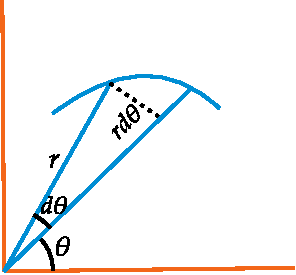
\includegraphics[height=4cm,width=5cm]{diagram-20220217(4)-20220217171419-crop}
	\caption{}
	\label{}
\end{figure}
If vector $\mathbf{r}$ rotates by an angle $d \theta$ in time $d t$, the area swept out by $r$ in time $d t$ is $\frac{1}{2} r .(r d \theta)=d A$ (say), so that
$$
\frac{d A}{d t}=\frac{1}{2} r^{2} \frac{d \theta}{d t}=\frac{1}{2} r^{2} \dot{\theta}
$$
From equation (\ref*{eq6});
\begin{align}
\frac{d A}{d t}=\frac{1}{2} r^{2} \dot{\theta}=\text { constant }
\end{align}
Equation (2.4) gives 
\begin{align*}
\frac{\partial L}{\partial \dot{r}}=\mu \dot{r}\\
\frac{\partial L}{\partial r}=\mu \dot{\theta}^{2}-\frac{\partial V}{\partial r} 
\end{align*}
The Lagrangian equation in terms of $r$ is given by
\begin{align}
\frac{d}{d t}\left(\frac{\partial L}{\partial \dot{r}}\right)-\frac{\partial L}{\partial r}=0 \notag\\
\frac{d}{d t}(\mu \dot{r})-\mu r \dot{\theta}^{2}+\frac{\partial V}{\partial r}=0\label{eq7}
\end{align}
If we represent the force along $\mathbf{r}$ by $F(r)$, then we have
$$
F(r)=-\frac{\partial V}{\partial r},
$$
so that equation \ref{eq7} can be written as
\begin{align}
\mu \ddot{r}-\mu r \dot{\theta}^{2}=F(r) \label{eq9}
\end{align}
This is the general equation of motion.\\
 But from equation (2.7),
 \begin{align*}
  \dot{\theta}=\frac{J}{\mu r^{2}}\\
 \dot{\theta}^{2}=\frac{J^{2}}{\mu^{2} r^{4}},
 \end{align*}
so that equation (\ref{eq9}) gives
\begin{align}
\mu \ddot{r}-\frac{J^{2}}{\mu r^{3}}=F(r) \label{eq10}
\end{align}
This is second order differential equation in $r$ only\\
 Equation (\ref{eq10}) gives\\
$
\mu \ddot{r}=\frac{J^{2}}{\mu r^{3}}+F(r),
$
\begin{align}
	&\mu \ddot{r}=\frac{j^{2}}{\mu r^{3}}-\frac{\partial V}{\partial r}=-\frac{1}{2} \frac{\partial}{\partial r}\left(\frac{J^{2}}{\mu r^{2}}\right)-\frac{\partial V}{\partial r} \notag \\
	&\mu \ddot{r}=-\frac{\partial}{\partial r}\left(\frac{1}{2} \frac{J^{2}}{\mu r^{2}}+V\right) \label{eq11}
\end{align}
Multiplying both sides of this equation by $\dot{r}$, we get
\begin{align*}
&\mu \dot{r} \ddot{r}=-\frac{\partial}{\partial r}\left(\frac{1}{2} \cdot \frac{J^{2}}{\mu r^{2}}+V\right) \dot{r} \\
&\frac{d}{d t}\left(\frac{1}{2} \mu \dot{r}^{2}\right)=-\frac{d}{d t}\left(\frac{1}{2} \frac{J^{2}}{\mu r^{2}}+V\right) \\
&\frac{d}{d t}\left(\frac{1}{2} \mu \dot{r}^{2}+\frac{1}{2} \frac{J^{2}}{\mu r^{2}}+V\right)=0 \\
&\frac{1}{2} \mu \dot{r}^{2}+\frac{1}{2} \frac{j^{2}}{\mu r^{2}}+V=\mathrm{constant}
\end{align*}
But
\begin{align*}
&\text { K.E. }=T=\frac{1}{2} \mu\left(\dot{r}^{2}+r^{2} \dot{\theta}^{2}\right) \\
&=\frac{1}{2} \mu\left(\dot{r}^{2}+\frac{J^{2}}{\mu^{2} r^{2}}\right) \\
&=\frac{1}{2} \mu \dot{r}^{2}+\frac{1}{2} \frac{J^{2}}{\mu r^{2}} \\
&\text { potential energy } =V\\
&\text { total energy } \quad E
=T+V=\frac{1}{2} \mu \dot{r}^{2}+\frac{1}{2} \frac{j^{2}}{\mu r^{2}}+V .
\end{align*}
From these equations we get 
\begin{align}
\frac{1}{2} \mu \dot{r}^{2}+\frac{1}{2} \mu^{2}+V=E=\text { constant } \label{eq12}
\end{align}
ie total energy of the system is constant ie the total energy E , constant of motion.This is the another first integral of motion .This equation (\ref{eq10}) represents equation of motion while angular momentum and total energy are constant of motion.\\
From equation (\ref{eq12}) we have
\begin{align}
	&\frac{1}{2} \mu \dot{r}^{2}=E-\frac{J^{2}}{2 \mu r^{2}}-V \notag\\
	&\dot{r}=\sqrt{\left[\frac{2}{\mu}\left\{E-\frac{J^{2}}{2 \mu r^{2}}-V\right\}\right]} \notag\\
	&\frac{d r}{d t}=\sqrt{\left[\frac{2}{\mu}\left(E-\frac{J^{2}}{2 \mu r^{2}}-V\right)\right]} \notag\\
	&\sqrt{\left[\frac{2}{\mu}\left(E-\frac{j^{2}}{2 \mu r^{2}}-V\right)\right]} \label{eq15}
\end{align}
$\text { Let the initial value of } r \text { be } r_{0} \text {; then integrating equation (\ref{eq15}), we get }$
\begin{align}
	&\int_{r_{\theta}}^{r} \frac{d r}{\sqrt{\left\{\frac{2}{\mu}\left(E-V-\frac{J^{2}}{2 \mu r^{2}}\right)\right\}}}=\int_{\theta}^{t} d t \notag \\
	&\left.t=\int_{r_{\theta}}^{r} \frac{d r}{\sqrt{\left\{\frac{2}{\mu}\left(E-V-\frac{J^{2}}{2 \mu r^{2}}\right)\right.}}\right\} \label{eq16}
\end{align}
This equation gives $t$ as a function of $r$. However, from this equation we can find $r$ as function of $t$ and the constants.
From equation (2.7), we have
$$
d \theta=\frac{J}{\mu r^{2}} d t
$$
If initially $\theta=\theta_{\theta}$, then integration of above equation yields
\begin{align}
&\int_{\theta_{0}}^{\theta} d \theta=\int_{0}^{t} \frac{J}{\mu r^{2}} d t \notag \\
&\theta-\theta_{0}=\int_{0}^{t} \frac{J}{\mu r^{2}} d t \notag \\
&\theta=\int_{0}^{1} \frac{J}{\mu r^{2}} d t+\theta_{0}
\end{align}
This equation gives $\theta$ as a function of $t$.\\
Equation(2.17 and 2.16) are the only integration to be solved .Therefore the problems have been reduced to quadratures with four constants $E,J,r_0,\theta_0$
\subsection{The equivalent one-dimensional problem, and classification of orbits}
Although we have solved the one dimensional problem formally ,practically speaking the integrals (1.16) and (1.17) are usually quite unmanageable and in specific case it is often more convenient to perform the integration in some other fashion.But before obtaining the solution for any specific force laws,let us see what can be learned about the motion in the general case using only the equation of motion and conservation theorems,without requiring explicit solutions.
\par The equation of motion in r,with $\dot{\theta}$ expressed in terms of l,quation     $m\ddot{r}-\frac{l^2}{mr^3}=f(r)$ involves only r and its derivatives.It is the same equation as would be obtained  for a fictitious one-dimensional problem in which a particle of mass $m$ is subject to a force
$$f^{\prime}=f+\frac{l^{2}}{m r^{3}}$$
The significance of the additional term is clear if it is written as $m r \dot{\theta}^{2}=m v_{\theta}^{2} / r$, which is the familiar centrifugal force. An equivalent statement can be obtained from the conservation theorem for energy. By Eq. $\frac{1}{2}m\dot{r}^2+\frac{1}{2}\frac{l^2}{mr^2}+V=constant$ the motion of the particle in $r$ is that of a one-dimensional problem with a fictitious potential energy:\\
$$V^{\prime}=V+\frac{1}{2} \frac{l^{2}}{m r^{2}}$$
As a check, note that
$$
f^{\prime}=-\frac{\partial V^{\prime}}{\partial r}=f(r)+\frac{l^{2}}{m r^{3}}
$$
 The energy conservation theorem can thus also be written as
$$
E=V^{\prime}+\frac{1}{2} m \dot{r}^{2}
$$
As an illustration of this method of examining the motion, consider a plot of $V^{\prime}$ against $r$ for the specific case of an attractive inverse-square law of force:
$$
f=-\frac{k}{r^{2}} .
$$
(For positive $k$, the minus sign ensures that the force is toward the center of force.) The potential energy for this force is
$$
V=-\frac{k}{r}
$$
and the corresponding fictitious potential is
$$
V^{\prime}=-\frac{k}{r}+\frac{l^{2}}{2 m r^{2}}
$$
Such a plot is shown in Figure the two dashed lines represent the separate components
$$
-\frac{k}{r} \quad \text { and } \quad \frac{l^{2}}{2 m r^{2}}
$$
and the solid line is the sum $V^{\prime}$.
\begin{figure}[H]
	\centering
	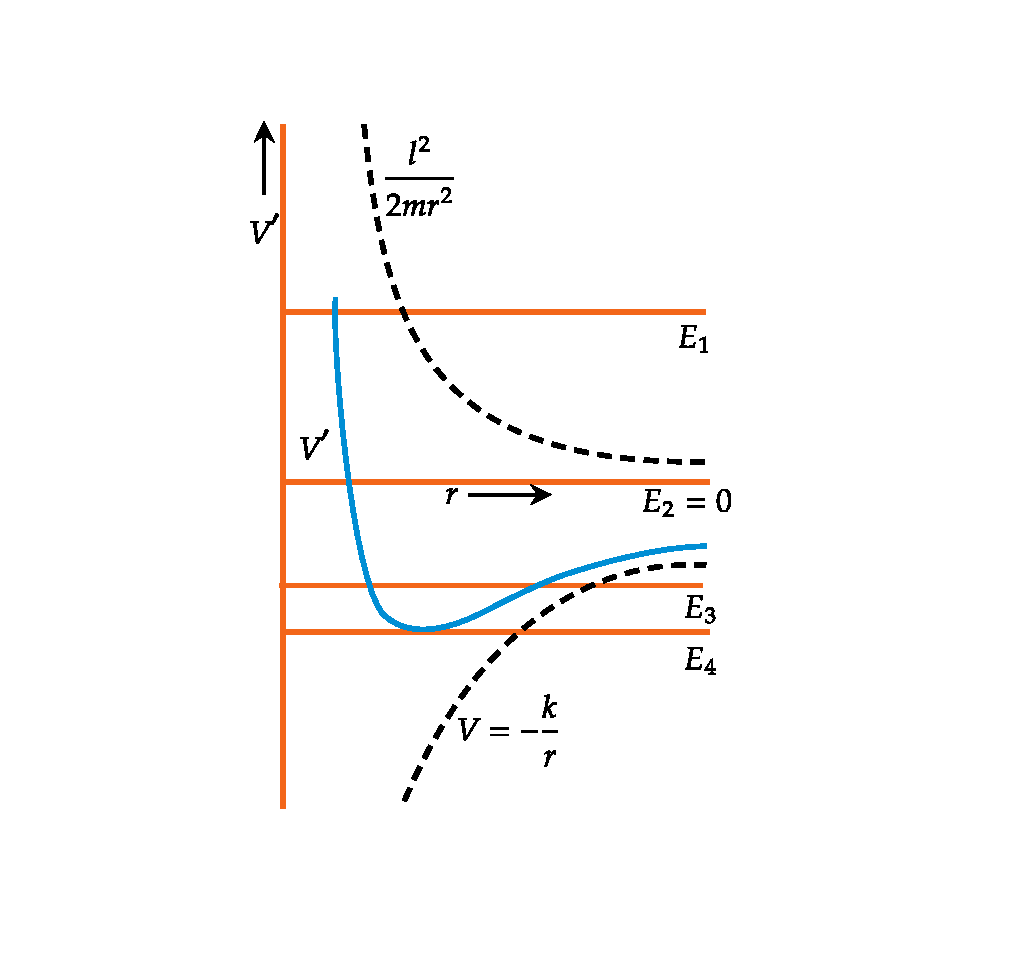
\includegraphics[height=9cm,width=9cm]{diagram-20220219(10)}
	\caption{The equivalent one dimensional potential for attractive inverse square law of force}
	\label{}
\end{figure}
Let us consider now the motion of a particle having the energy $E_{1}$, as shown in Figures. Clearly this particle can never come closer than $r_{1}$  Otherwise with $r<r_{1}, V^{\prime}$ exceeds $E_{1}$ and by conservation of energy the kinetic energy would have to be negative, corresponding to an imaginary velocity! on the other hand, there is no upper limit to the possible value of $r$, so the orbit is not bounded. A particle will come in from infinity, strike the "repulsive centrifugal barrier," be repelled, and travel back out to infinity. The distance between $E$ and $V^{\prime}$ is $\frac{1}{2} m \dot{r}^{2}$, i.e., proportional to the square of the radial velocity, and becomes zero, naturally, at the turning point $r_{1}$. At the same time. the distance between $E$ and $V$ on the plot is the kinetic energy $\frac{1}{2} m v^{2}$ at the given value of $r$. Hence, the distance between the $V$ and $V^{\prime}$ curves is $\frac{1}{2} m r^{2} \theta^{2}$. These curves therefore supply the magnitude of the particle velocity and its components for any distance r,at the given energy and angular momentum .This information is sufficient to produce an approximate picture of the form of the orbit.\\
\begin{minipage}{0.5\textwidth}
\begin{figure}[H]
	\centering
	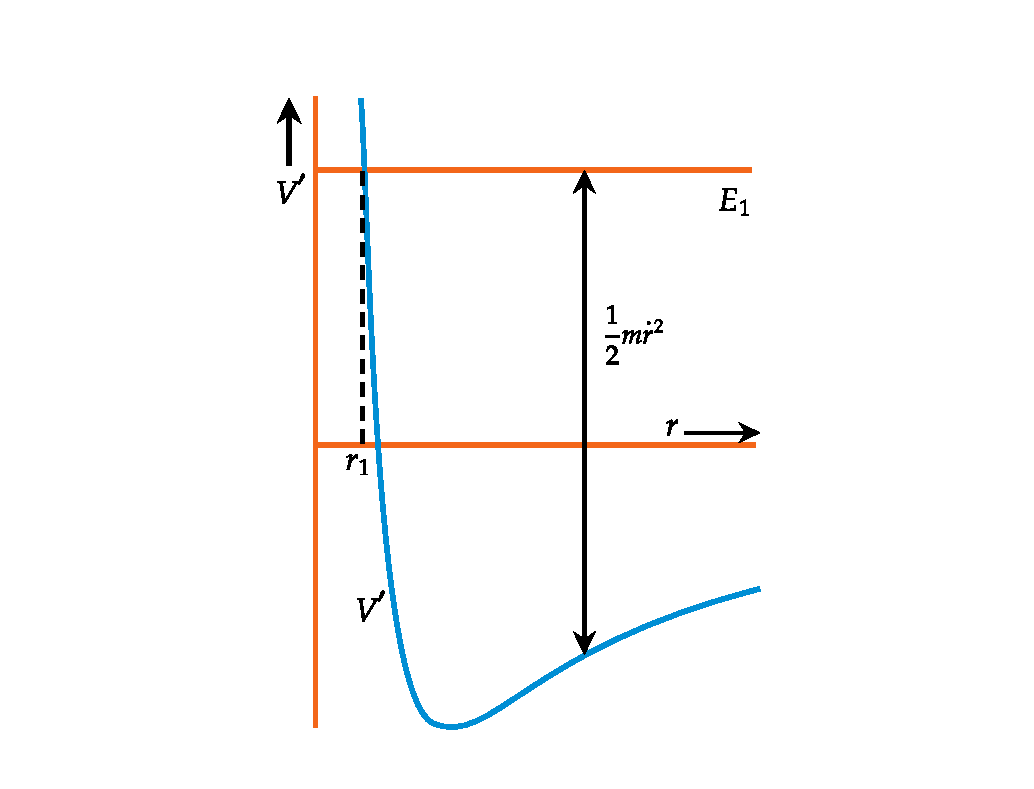
\includegraphics[height=7cm,width=10cm]{diagram-20220219(11)}
	\caption{Unbounded motion at positive energies for inverse square law of force}
	\label{}
\end{figure}
\end{minipage}
\begin{minipage}{0.5\textwidth}
\begin{figure}[H]
	\centering
	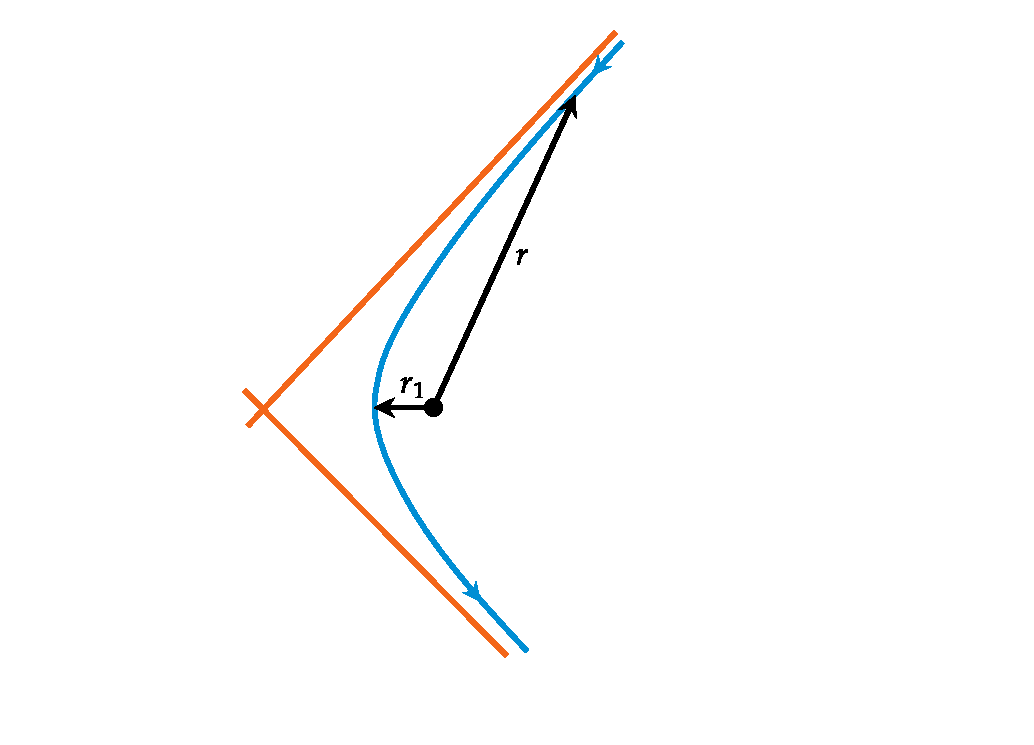
\includegraphics[height=5cm,width=7cm]{diagram-20220219(6)}
	\caption{The orbit for $E_1$ corresponding to unbounded motion}
	\label{}
\end{figure}
\end{minipage}
\par For the energy $E_{2}=0$, a roughly similar picture of the orbit behavior is obtained. But for any lower energy, such as $E_{3}$ indicated in fig (1.6) we have a different story. In addition to a lower bound $r_{1}$, there is also a max. imum value $r_{2}$ that cannot be exceeded by $r$ with positive kinetic energy. The motion is then "bounded," and there are two turning points, $r_{1}$ and $r_{2}$, also known as apsidal distances. This does not necessarily mean that the orbits are closed. All that can be said is that they are bounded, contained between two circles of radius $r_{1}$ and $r_{2}$ with turning points always lying on the circles\\
\begin{minipage}{0.5\textwidth}
	\begin{figure}[H]
		\centering
		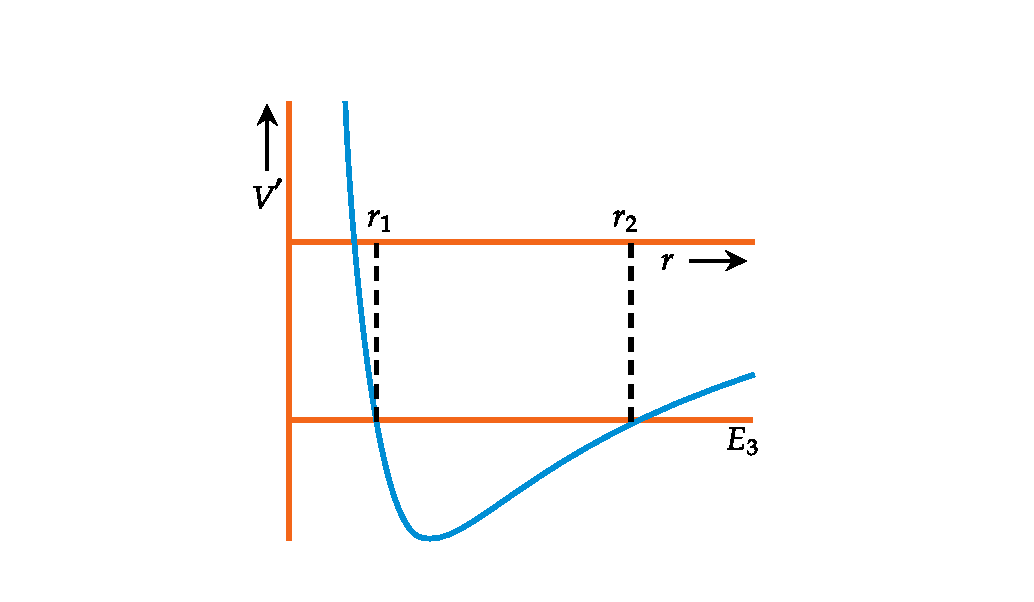
\includegraphics[height=8cm,width=9cm]{diagram-20220219(8)}
		\caption{The equivalent one dimensional potential for inverse square law of force illustrating bounded motion at negative energies.}
		\label{}
	\end{figure}
\end{minipage}
\begin{minipage}{0.5\textwidth}
\begin{figure}[H]
	\centering
	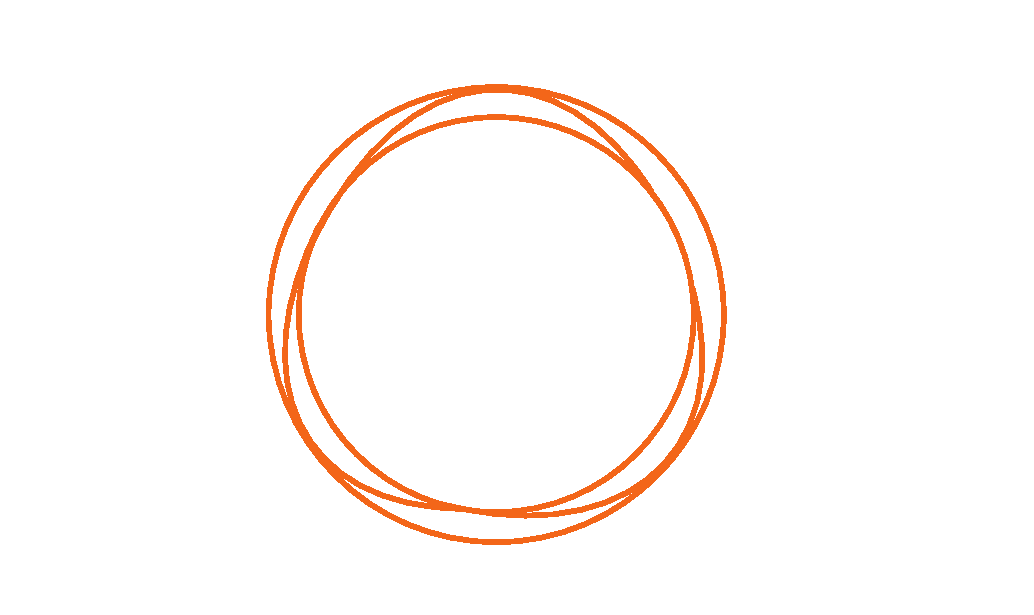
\includegraphics[height=5cm,width=7cm]{diagram-20220219(7)}
	\caption{The nature of the orbit for bounded motion}
	\label{}
\end{figure}
\end{minipage}
\par If the energy is $E_{4}$ at the minimum of the fictitious potential as shown in Fig. (1.8), then the two bounds coincide. In such case, motion is possible at only one radius; $\dot{r}=0$, and the orbit is a circle.
\begin{figure}[H]
	\centering
	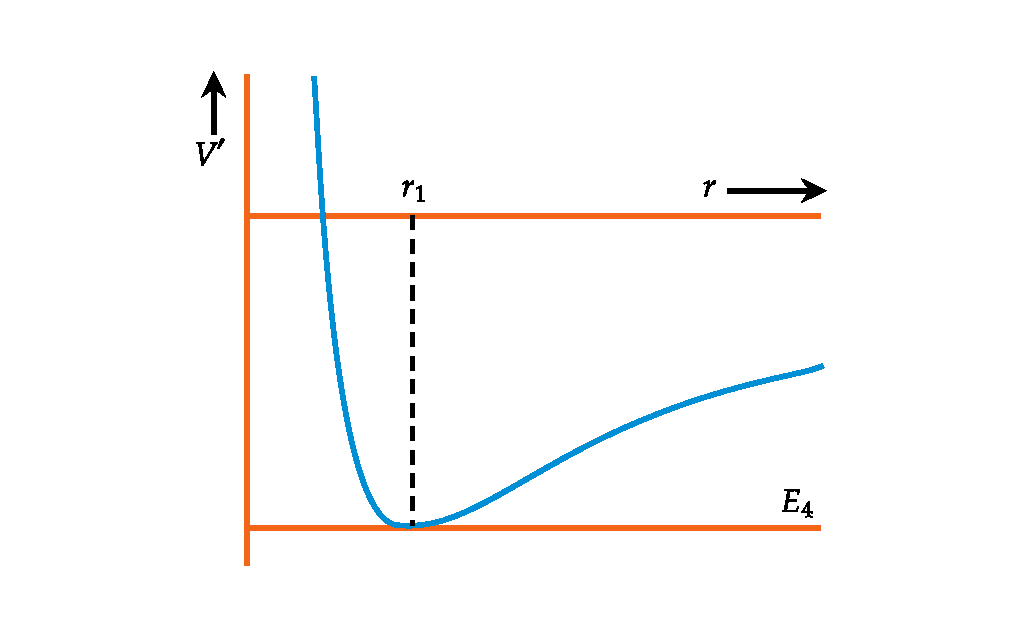
\includegraphics[height=7cm,width=7cm]{diagram-20220219(9)}
	\caption{The equivalent one dimensional potential of inverse square law of force,illustrating the condition for circular orbits}
	\label{}
\end{figure}
\begin{note}
Remembering that the effective "force" is the negative of the slope of the $V^{\prime}$ curve, the requirement for circular orbits is simply that $f^{\prime}$ be zero, or
$$
f(r)=-\frac{l^{2}}{m r^{3}}=-m r \dot{\theta}^{2}
$$
which can be also derived by $\left.\frac{\partial V_{\text {effective }}}{\partial r}\right|_{r=r_{0}}=0$ and $\dot{\theta}=\omega_{0}$ is identified as angular frequency circular orbit.	
\end{note}
\subsection{The differential equation for the orbit}
Under central force
\begin{align}
\text{We have }J=\mu r^{2} \dot{\theta}= \text{constant}\\
and E=\frac{1}{2} \mu \dot{r}^{2}+\frac{J^{2}}{2 \mu r^{2}}+V= \text{constant}\\
\text{Differential equation in r is} \notag\\
\mu \ddot{r}-\frac{J^{2}}{\mu r^{3}}=F(r)
\end{align}
From equation (2.18)
\begin{align}
	&J=\mu r^{2} \dot{\theta}\notag  \\
	&J=\mu r^{2} \frac{d \theta}{d t}\notag \\ 
	&J d t=\mu r^{2} d \theta
\end{align}
The corresponding relation between the derivative relative to $t$ and $\theta$ can be written as
\begin{align}
\frac{d}{d t}=\frac{J}{\mu r^{2}} \frac{d}{d \theta}
\end{align}
second derivative w.r.t. t can be written as \\
\begin{equation}
\frac{d^{2}}{d t^{2}}=\frac{J}{\mu r^{2}} \frac{d}{d \theta}\left[\frac{J}{\mu r^{2}} \frac{d}{d \theta}\right]
\end{equation}
from equation (2.20)\\
\begin{align}
	&\mu \frac{J}{\mu r^{2}} \frac{d}{d \theta}\left\{\frac{J}{\mu r^{2}} \frac{d r}{d \theta}\right\}-\frac{J^{2}}{\mu r^{3}}=F(r) . \notag \\
	&\frac{J}{r^{2}} \frac{d}{d \theta}\left\{\frac{J}{\mu r^{2}} \frac{d r}{d \theta}\right\}-\frac{J^{2}}{\mu r^{3}}=F(r)
\end{align}
To simplify above equation we must remember that
\begin{equation}
\frac{1}{r^{2}} \frac{d r}{d \theta}=-\frac{d(1 / r)}{d \theta}
\end{equation}
$\text { Using }(2.25) \text {, equation (2.24) gives }$\\
\begin{equation}
\frac{J^{2}}{\mu r^{2}} \frac{d}{d \theta}\left[-\frac{d(1 / r)}{d \theta}\right]-\frac{J^{2}}{\mu r^{3}}=F(r)
\end{equation}
Substituting
$$
u=\frac{1}{r}
$$
equation (2.26) gives \\
\begin{align}
	&-\frac{J^{2} u^{2} d^{2} u}{\mu} \frac{J^{2}}{\mu^{2}}-\frac{J^{2}}{\mu}=F\left(\frac{1}{u}\right) \notag \\
	&\frac{J^{2} u^{2}}{\mu}\left[\frac{d^{2} u}{d \theta^{2}}+u\right]=-F\left(\frac{1}{u}\right)
\end{align}
This is the differential equation for the orbit if the force F is known.
\subsection{The kepler problem:Inverse square law of force}
The inverse square law is most important of all central force laws.It results in the deduction of Kepler's laws of planetary motion.\\
\textbf{The kepler's laws of planetary motion are:}\\
(i) All planets move in elliptical orbits having the sun as one focus.\\
(ii)The area swepts out by the radius vector of planet relative to the sun in equal times are equal.\\
(iii)The square of the period of revolution of any planet about the sun is proportional to the cube of the semi major axis\\
\textbf{Deduction of Kepler's laws}\\
\textbf{Kepler's first law}\\
Under central force the constant of motion are angular momentum and energy
\begin{align}
J&=\mu r^{2} \dot{\theta} \\
 E&=\frac{1}{2} \mu \dot{r}^{2}+\frac{J^{2}}{2 \mu r^{2}}+V
\end{align}
From equation (2.28 and 2.29)\\
\begin{align}
	&\frac{d \theta}{d t}=\frac{J}{\mu r^{2}} \\
	&\frac{d r}{d t}=\sqrt{\frac{2}{\mu}\left(E-\frac{J^{2}}{2 \mu r^{2}}-V\right)}
\end{align}
Dividing equation (2.31) by (2.30)
\begin{align}
	\frac{dr}{d \theta} &=\frac{\mu r^{2}}{J} \times \sqrt{\left\{\frac{2}{\mu}\left(E-V-\frac{j^{2}}{2 \mu r^{2}}\right)\right\}} \\
	d \theta &=\frac{J d r}{\mu r^{2} \sqrt{\left\{\frac{2}{\mu}\left(E-V-\frac{J^{2}}{2 \mu r^{2}}\right)\right\}}}
\end{align}
Under inverse square law of force, we have

\begin{align*}
&F(r)=-\frac{k}{r^{2}} \\
&F(r)=-\frac{\partial V}{\partial r} \\
&-\frac{\partial V}{\partial r}=-\frac{k}{r^{2}} \Rightarrow d V=\frac{k}{r^{2}} d r
\end{align*}
Integrating $\quad V=\int^{r} \frac{k}{r^{2}} d r$\\
or the potential energy $V=-\frac{k}{r}$.\\
Substituting this value of $V$ in equation (2.33), we get
$$
d \theta=\frac{J d r}{\sqrt[\mu r^{2}]{\left\{\frac{2}{\mu}\left(E+\frac{k}{r}-\frac{J^{2}}{2 \mu r^{2}}\right)\right\}}}
$$
Integrating, we get
$$
\theta=\int \frac{J d r}{\mu r^{2} \sqrt{\left\{\frac{2}{\mu}\left(E+\frac{k}{r}-\frac{J^{2}}{2 \mu r^{2}}\right)\right\}}}+\theta^{\prime}
$$
where $\theta^{\prime}$ is constant of integration.\\
Substituting $r=1 / u$, we get\\
\begin{align}
\theta=-\int \frac{J d u}{\mu \sqrt{\left\{\frac{2}{\mu}\left(E+k u-\frac{J^{2} u^{2}}{2 \mu}\right)\right\}}}+\theta^{\prime} \notag \\
=\theta^{\prime}-\int \frac{d u}{\sqrt{\left(\frac{2 \mu E}{J^{2}}+\frac{2 \mu k u}{J^{2}}-u^{2}\right)}} \notag \\
=\theta^{\prime}-\int \frac{d u}{\sqrt{\left[\left(\frac{2 \mu E}{J^{2}}+\frac{\mu^{2} k^{2}}{J^{4}}\right)-\left(u-\frac{\mu k}{J^{2}}\right)^{2}\right]}} \notag\\
=\theta^{\prime}-\cos ^{-1} \frac{u-\frac{\mu k}{J^{2}}}{\sqrt{\left(\frac{2 \mu E}{J^{2}}+\frac{\mu^{2} k^{2}}{J^{4}}\right)}}=\theta^{\prime}-\cos ^{-1} \frac{\frac{u J^{2}}{\mu k}-1}{\sqrt{\left(\frac{2 E J^{2}}{\mu k^{2}}+1\right)}} \notag\\
\frac{\frac{u J^{2}}{\mu k}-1}{\sqrt{\left(\frac{2 E J^{2}}{\mu k^{2}}+1\right)}}=\cos \left(\theta-\theta^{\prime}\right)\notag\\
\frac{u J^{2}}{\mu k}-1=\sqrt{\left(\frac{2 E J^{2}}{\mu k^{2}}+1\right)} \cos \left(\theta-\theta^{\prime}\right) \notag \\
u=\frac{\mu k}{J^{2}}\left[1+\sqrt{\left(\frac{2 E J^{2}}{\mu k^{2}}+1\right)} \cos \left(\theta-\theta^{\prime}\right)\right]
\end{align}
Substituting
\begin{align}
c &=\frac{\mu k}{J^{2}} \\
\varepsilon &=\sqrt{\left(1+\frac{2 E J^{2}}{\mu k^{2}}\right)}
\end{align}
Equation (2.34) gives\\
\begin{align}
	u &=c\left[1+\varepsilon \cos \left(\theta-\theta^{\prime}\right)\right] \notag \\
	\frac{1}{r} &=c\left[1+\varepsilon \cos \left(\theta-\theta^{\prime}\right)\right]
\end{align}
which is the equation of the conic with $\varepsilon$ as eccentricity and one focus as the origin. Thus the equation of the path of the two-body problem of reduced mass $\mu$ is always a conic section, which is the generalisation of Kepler's first law.\\
The nature of the conic dependes on the value of eccentricity given by eqn. (2.36).\\
 If $\in>1$, i.e., if $\sqrt{\left(\frac{2 E J^{2}}{\mu k^{2}}+1\right)}>1$ or $E>0$, the conic is hyperbola.\\
 If $\in=1$, i.e., if $\sqrt{\left(\frac{2 E J^{2}}{\mu k^{2}}+1\right)}=1$ or $E=0$, the conic is a parabola.\\
  If $\in<1$, i.e., if $\sqrt{\left(\frac{2 E^{2}}{\mu k^{2}}+1\right)}<1$ or $E<0$, the conic is an ellipse.\\
   If $\in=0$, i.e., if $\sqrt{\left(\frac{2 E^{2}}{\mu k^{2}}+1\right)}=0$ or $E=-\frac{\mu k^{2}}{2 J^{2}}$, the conic is a circle.\\
    In the case of elliptical orbits, when $\theta-\theta^{\prime}=0, r=r_{1}=$ perihelion,\\
    \begin{figure}[H]
    	\centering
    	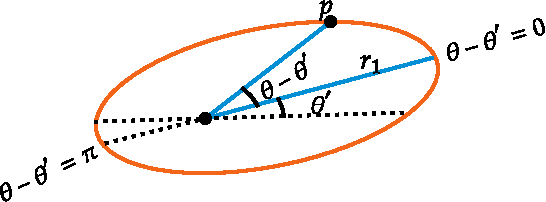
\includegraphics[height=4cm,width=7cm]{diagram-20220217(3)-20220217170838-crop}
    	\caption{}
    	\label{}
    \end{figure}
    Then from equation (2.37) we have\\
    $$r_{1}=\frac{1}{c(1+\varepsilon)}$$
    When $\theta-\theta^{\prime}=\pi, r=r_{2}=$ aphelion, then eqn. (2.37) gives
    $$
    r_{2}=\frac{1}{c(1-\varepsilon)}
    $$
    The semi-major axis, which is one-half the sum of perihelion $r_{1}$ and aphelion $r_{2}$ is given by
    $$a=\frac{r_{1}+r_{2}}{2}=\frac{1}{2}\left[\frac{1}{c(1+\varepsilon)}+\frac{1}{c(1-\varepsilon)}\right]$$
    Substituting values of $c$ and $\varepsilon$ , we get
    \begin{align}
    &a=\frac{1}{\frac{\mu k}{J^{2}}\left\{1-\left(1+\frac{2 E J^{2}}{\mu k^{2}}\right)\right\}}=-\frac{k}{2 E} \notag \\
    &E=-\frac{k}{2 a} .
    \end{align}
  This shows that in the case of elliptical orbits the total energy depends solely on the major axis.\\
  \textbf{Deduction of II law}\\
  $$J=\mu r^{2} \dot{\theta}=\text { constant }$$
  This implies
  $$
  \frac{d A}{d t}=\frac{1}{2} r^{2} \dot{\theta}=\text { constant }
  $$
  which represents the areal velocity, i.e., the area swept out by the radius vector per unit time is constant. This means that the areas swept out by the radius vector in equal times are equal which is Kepler's II law.\\
  \textbf{Deduction of kepler's III Law}\\
If $T$ is the periodic time of describing the complete orbit, the area of the orbit is given by\\
\begin{align}
A &=\int_{0}^{T} \frac{d A}{d t} d t=\int_{0}^{T} \frac{1}{2} r^{2} \ddot{\theta} d t \notag \\
&=\int_{0}^{T} \frac{J}{2 \mu} d t \quad\left(\text { since } J=\mu r^{2} \dot{\theta}\right) \notag \\
&=\frac{J T}{2 \mu}
\end{align}
But area of the ellipse 
\begin{equation}
\mathrm{A}=\pi a b
\end{equation}
where $a$ and $b$ are the semi-major and semi-minor axes of the ellipse respectively.
$$
\begin{array}{ll}
\text { Also } & b=a \sqrt{\left(1-\varepsilon^{2}\right)}=a \sqrt{\left(1-1-\frac{2 E J^{2}}{\mu k^{2}}\right)}=a \sqrt{\left(-\frac{2 E J^{2}}{\mu k^{2}}\right)} \\
\text { But } & E=-\frac{k}{2 a}
\end{array}
$$
Therefore
\begin{equation}
b=a \sqrt{\left(\frac{k J^{2}}{a \mu k^{2}}\right)}=a^{1 / 2} \sqrt{\left(\frac{J^{2}}{\mu k}\right)}
\end{equation}
Substituting value of $b$ in equation (2.40) we get
\begin{equation}
A=\pi a^{3 / 2} \sqrt{\left(\frac{J^{2}}{\mu k}\right)}
\end{equation}
Comparing equation (2.39 and 2.42)\\
\begin{align}
	&\frac{J T}{2 \mu}=\pi a^{3 / 2} \sqrt{\left(\frac{J^{2}}{\mu k}\right)} \notag \\
	&\frac{J^{2} T^{2}}{4 \mu^{2}}=\pi^{2} a^{3} \frac{J^{2}}{\mu k} \notag \\
	&T^{2}=4 \pi^{2} a^{3} \frac{\mu}{k} \notag \\
	&T^{2} \propto a^{3}
\end{align}
ie the square of the period of revolution of the planet around the sun is proportional to the cube of the semimajor axis, which is kepler's III law.
\section{Two body collisions}
When discussing conservation of momentum, we considered examples in which two
objects collide and stick together, and either there are no external forces acting in some
direction (or the collision was nearly instantaneous) so the component of the momentum
of the system along that direction is constant. We shall now study collisions between
objects in more detail. In particular we shall consider cases in which the objects do not
stick together. The momentum along a certain direction may still be constant but the
mechanical energy of the system may change. We will begin our analysis by considering
two-particle collision. We introduce the concept of the relative velocity between two
particles and show that it is independent of the choice of reference frame. We then show
that the change in kinetic energy only depends on the change of the square of the relative
velocity and therefore is also independent of the choice of reference frame. We will then
study one- and two-dimensional collisions with zero change in potential energy. In
particular we will characterize the types of collisions by the change in kinetic energy and analyze the possible outcomes of the collisions.
\subsection{Laboratary frame of reference}
 Let $\overrightarrow{\mathbf{R}}$ be the vector from the origin of frame $S$ to the origin of reference frame $S^{\prime}$. Denote the position vector of the $j^{\text {th }}$ particle with respect to the origin of reference frame $S$ by $\overrightarrow{\mathbf{r}}_{j}$ and similarly, denote the position vector of the $j^{\text {th }}$ particle with respect to the origin of reference frame $S^{\prime}$ by $\overrightarrow{\mathbf{r}}_{j}^{\prime}$ .\\
 \begin{figure}[H]
 	\centering
 	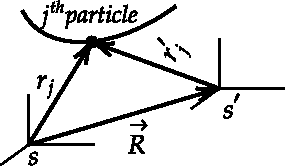
\includegraphics[height=3cm,width=5cm]{diagram-20220218-crop}
 	\caption{}
 	\label{}
 \end{figure}
The position vectors are related by
$$
\overrightarrow{\mathbf{r}}_{j}=\overrightarrow{\mathbf{r}}_{j}^{\prime}+\overrightarrow{\mathbf{R}}
$$
The relative velocity (call this the boost velocity) between the two reference frames is given by
$$
\overrightarrow{\mathbf{V}}=\frac{d \overrightarrow{\mathbf{R}}}{d t}
$$
Assume the boost velocity between the two reference frames is constant. Then, the relative acceleration between the two reference frames is zero,
$$
\overrightarrow{\mathbf{A}}=\frac{d \overrightarrow{\mathbf{V}}}{d t}=\overrightarrow{\mathbf{0}}
$$
When the equation is satisfied, the reference frames $S$ and $S^{\prime}$ are called relatively inertial reference frames.\\
Suppose the $j^{\text {th }}$ particle in Figure is moving; then observers in different reference frames will measure different velocities. Denote the velocity of $j^{\text {th }}$ particle in frame $S$ by $\overrightarrow{\mathbf{v}}_{j}=d \overrightarrow{\mathbf{r}}_{j} / d t$, and the velocity of the same particle in frame $S^{\prime}$ by $\overrightarrow{\mathbf{v}}_{j}^{\prime}=d \overrightarrow{\mathbf{r}}_{j}^{\prime} / d t$. Taking derivative, the velocities of the particles in two different reference frames are related according to
$$
\overrightarrow{\mathbf{v}}_{j}=\overrightarrow{\mathbf{v}}_{j}^{\prime}+\overrightarrow{\mathbf{V}}
$$
\subsection{ Center-of-mass Reference Frame}
Let $\overrightarrow{\mathbf{r}}_{c m}$ be the vector from the origin of frame $S$ to the center-of-mass of the system of particles, a point that we will choose as the origin of reference frame $S_{c m}$, called the center-of-mass reference frame. Denote the position vector of the $j^{\text {th }}$ particle with respect to origin of reference frame $S$ by $\overrightarrow{\mathbf{r}}_{j}$ and similarly, denote the position vector of the $j^{\text {th }}$ particle with respect to origin of reference frame $S_{c m}$ by $\overrightarrow{\mathbf{r}}_{j}^{\prime}$ \\
\begin{figure}[H]
	\centering
	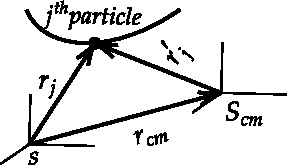
\includegraphics[height=3cm,width=5cm]{diagram-20220218(1)-crop}
	\caption{}
	\label{}
\end{figure}
The position vector of the $j^{\text {th }}$ particle in the center-of-mass frame is then given by
$$
\overrightarrow{\mathbf{r}}_{j}^{\prime}=\overrightarrow{\mathbf{r}}_{j}-\overrightarrow{\mathbf{r}}_{c m} .
$$
The velocity of the $j^{\text {th }}$ particle in the center-of-mass reference frame is then given by
$$
\overrightarrow{\mathbf{v}}_{j}^{\prime}=\overrightarrow{\mathbf{v}}_{j}-\overrightarrow{\mathbf{v}}_{c m}
$$
There are many collision problems in which the center-of-mass reference frame is the most convenient reference frame to analyze the collision.\\
Consider a system consisting of two particles, which we shall refer to as particle 1 and particle $2 .$ We can determine the velocities of particles 1 and 2 in the center-of-mass,
as\\\\
$$\overrightarrow{\mathbf{v}}_{1}^{\prime}=\overrightarrow{\mathbf{v}}_{1}-\overrightarrow{\mathbf{v}}_{c m}=\overrightarrow{\mathbf{v}}_{1}-\frac{m_{1} \overrightarrow{\mathbf{v}}_{1}+m_{2} \overrightarrow{\mathbf{v}}_{2}}{m_{1}+m_{2}}=\frac{m_{2}}{m_{1}+m_{2}}\left(\overrightarrow{\mathbf{v}}_{1},-\overrightarrow{\mathbf{v}}_{2}\right)=\frac{\mu}{m_{1}} \overrightarrow{\mathbf{v}}_{1,2}$$
where $\overrightarrow{\mathbf{v}}_{12}=\overrightarrow{\mathbf{v}}_{1}-\overrightarrow{\mathbf{v}}_{2}$ is the relative velocity of particle 1 with respect to particle 2 . A similar result holds for particle 2 :\\\\
$$\overrightarrow{\mathbf{v}}_{2}^{\prime}=\overrightarrow{\mathbf{v}}_{2}-\overrightarrow{\mathbf{v}}_{c m}=\overrightarrow{\mathbf{v}}_{2}-\frac{m_{1} \overrightarrow{\mathbf{v}}_{1}+m_{2} \overrightarrow{\mathbf{v}}_{2}}{m_{1}+m_{2}}=-\frac{m_{1}}{m_{1}+m_{2}}\left(\overrightarrow{\mathbf{v}}_{1}-\overrightarrow{\mathbf{v}}_{2}\right)=-\frac{\mu}{m_{2}} \overrightarrow{\mathbf{v}}_{1,2}$$
The momentum of the system the center-of-mass reference frame is zero as we expect,
$$
m_{1} \overrightarrow{\mathbf{v}}_{1}^{\prime}+m_{2} \overrightarrow{\mathbf{v}}_{2}^{\prime}=\mu \overrightarrow{\mathbf{v}}_{12}-\mu \overrightarrow{\mathbf{v}}_{12}=\overrightarrow{\mathbf{0}}
$$
\subsection{ Characterizing Collisions}
In a collision, the ratio of the magnitudes of the initial and final relative velocities is called the coefficient of restitution and denoted by the symbol $e$,
$$
e=\frac{v_{B}}{v_{A}}
$$
If the magnitude of the relative velocity does not change during a collision, $e=1$, then the change in kinetic energy is zero. Collisions in which there is no change in kinetic energy are called elastic collisions,
$$\Delta K=0, \text{elastic collision }$$
If the magnitude of the final relative velocity is less than the magnitude of the initial relative velocity, $e<1$, then the change in kinetic energy is negative. Collisions in which the kinetic energy decreases are called inelastic collisions,
$$\Delta K<0, \text{inelastic collision }$$
If the two objects stick together after the collision, then the relative final velocity is zero, $e=0 .$ Such collisions are called totally inelastic. The change in kinetic energy can be written as\\
$$\Delta K=-\frac{1}{2} \mu v_{A}^{2}=-\frac{1}{2} \frac{m_{1} m_{2}}{m_{1}+m_{2}} v_{A}^{2}, \text { totally inelastic collision } .$$
If the magnitude of the final relative velocity is greater than the magnitude of the initial relative velocity, $e>1$, then the change in kinetic energy is positive. Collisions in which the kinetic energy increases are called superelastic collisions,
$$\Delta K>0, \textbf{superelastic collision}$$
\subsection{ Two-dimensional Elastic Collision in Laboratory Reference Frame}
Consider the elastic collision between two particles in which we neglect any external forces on the system consisting of the two particles. Particle 1 of mass $m_{1}$ is initially moving with velocity $\overrightarrow{\mathbf{v}}_{1, i}$ and collides elastically with a particle 2 of mass $m_{2}$ that is initially at rest. We shall refer to the reference frame in which one particle is at rest, 'the target', as the laboratory reference frame. After the collision particle 1 moves with velocity $\overrightarrow{\mathbf{v}}_{1, f}$ and particle 2 moves with velocity $\overrightarrow{\mathbf{v}}_{2, f}$, (Figure). The angles $\theta_{1, f}$ and $\theta_{2, f}$ that the particles make with the positive forward direction of particle 1 are called the laboratory scattering angles.\\
\begin{figure}[H]
	\centering
	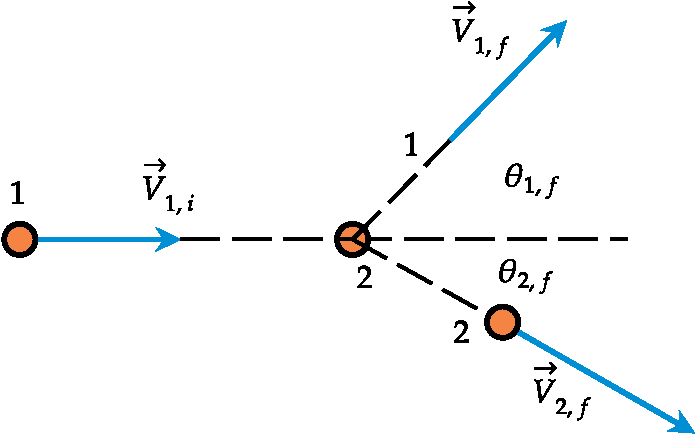
\includegraphics[height=5cm,width=8cm]{class20}
	\caption{}
	\label{}
\end{figure}
Generally the initial velocity $\overrightarrow{\mathbf{v}}_{1, i}$ of particle 1 is known and we would like to determine the final velocities $\overrightarrow{\mathbf{v}}_{1, f}$ and $\overrightarrow{\mathbf{v}}_{2, f}$, which requires finding the magnitudes and directions of each of these vectors, $v_{1, f}, v_{2, f}, \theta_{1, f}$, and $\theta_{2, f} .$ These quantities are related by the two equations describing the constancy of momentum, and the one equation describing constancy of the kinetic energy. Therefore there is one degree of freedom that we must specify in order to determine the outcome of the collision. In what follows we shall express our results for $v_{1, f}, v_{2, f}$, and $\theta_{2, f}$ in terms of $v_{1, i}$ and $\theta_{1, f}$.\\
The components of the total momentum $\overrightarrow{\mathbf{p}}_{i}^{\mathrm{sys}}=m_{1} \overrightarrow{\mathbf{v}}_{1, i}+m_{2} \overrightarrow{\mathbf{v}}_{2, i}$ in the initial state are given by
$$
\begin{aligned}
p_{x, i}^{\mathrm{sys}} &=m_{1} v_{1, i} \\
p_{y, i}^{\mathrm{sys}} &=0 .
\end{aligned}
$$
The components of the momentum $\overrightarrow{\mathbf{p}}_{f}^{\mathrm{sys}}=m_{1} \overrightarrow{\mathbf{v}}_{1, f}+m_{2} \overrightarrow{\mathbf{v}}_{2, f}$ in the final state are given by
$$
\begin{aligned}
&p_{x, f}^{\mathrm{sys}}=m_{1} v_{1, f} \cos \theta_{1, f}+m_{2} v_{2, f} \cos \theta_{2, f} \\
&p_{y, f}^{\mathrm{sys}}=m_{1} v_{1, f} \sin \theta_{1, f}-m_{2} v_{2, f} \sin \theta_{2, f} .
\end{aligned}
$$
There are no any external forces acting on the system, so each component of the total momentum remains constant during the collision,
$$
\begin{aligned}
&p_{x, i}^{\text {sys }}=p_{x, f}^{\text {sys }} \\
&p_{y, i}^{\text {sys }}=p_{y, f}^{\text {sy }}
\end{aligned}
$$
substituting the values\\
$$\begin{gathered}
m_{1} v_{1, i}=m_{1} v_{1, f} \cos \theta_{1, f}+m_{2} v_{2, f} \cos \theta_{2, f} \\
0=m_{1} v_{1, f} \sin \theta_{1, f}-m_{2} v_{2, f} \sin \theta_{2, f}
\end{gathered}$$
rewriting the expressions we will get \\
\begin{align}
m_{2} v_{2, f} \cos \theta_{2, f}=m_{1}\left(v_{1, i}-v_{1, f} \cos \theta_{1, f}\right)\\
m_{2} v_{2, f} \sin \theta_{2, f}=m_{1} v_{1, f} \sin \theta_{1, f}
\end{align}
Squaring and adding and using the identity $\text { the identity } \cos ^{2} \theta+\sin ^{2} \theta=1 \text { yielding }$
$$v_{2, f}^{2}=\frac{m_{1}^{2}}{m_{2}^{2}}\left(v_{1, i}^{2}-2 v_{1, i} v_{1, f} \cos \theta_{1, f}+v_{1, f}^{2}\right)$$
The collision is elastic and therefore the system kinetic energy of is constant
$$
K_{i}^{\text {sys }}=K_{f}^{\text {sys }}
$$
$$
\frac{1}{2} m_{1} v_{1, i}^{2}=\frac{1}{2} m_{1} v_{1, f}^{2}+\frac{1}{2} m_{2} v_{2, f}^{2}
$$
substituting the value of $v_{2, f}^{2}$ in this equation\\
$$\frac{1}{2} m_{1} v_{1, i}^{2}=\frac{1}{2} m_{1} v_{1, f}^{2}+\frac{1}{2} \frac{m_{1}^{2}}{m_{2}}\left(v_{1, i}^{2}-2 v_{1, i} v_{1, f} \cos \theta_{1, f}+v_{1, f}^{2}\right)$$
$$0=\left(1+\frac{m_{1}}{m_{2}}\right) v_{1, f}^{2}-\frac{m_{1}}{m_{2}} 2 v_{1, i} v_{1, f} \cos \theta_{1, f}-\left(1-\frac{m_{1}}{m_{2}}\right) v_{1, i}^{2}$$
Let $\alpha=m_{1} / m_{2}$ then Equation can be written as
$$
0=(1+\alpha) v_{1, f}^{2}-2 \alpha v_{1, i} v_{1, f} \cos \theta_{1, f}-(1-\alpha) v_{1, i}^{2}
$$
The solution to this quadratic equation is given by
$$
v_{1, f}=\frac{\alpha v_{1, i} \cos \theta_{1, f} \pm\left(\alpha^{2} v_{1, i}^{2} \cos ^{2} \theta_{1, f}+(1-\alpha) v_{1, i}^{2}\right)^{1 / 2}}{(1+\alpha)}
$$
Divide equation (2.44 and 2.25) yields\\
$$\begin{gathered}
\frac{v_{2, f} \sin \theta_{2, f}}{v_{2, f} \cos \theta_{2, f}}=\frac{v_{1, f} \sin \theta_{1, f}}{v_{1, i}-v_{1, f} \cos \theta_{1, f}} \\
\tan \theta_{2, f}=\frac{v_{1, f} \sin \theta_{1, f}}{v_{1, i}-v_{1, f} \cos \theta_{1, f}} .
\end{gathered}$$
The relationship between the scattering angles is independent of the masses of the colliding particles. Thus the scattering angle for particle 2 is
$$\theta_{2, f}=\tan ^{-1}\left(\frac{v_{1, f} \sin \theta_{1, f}}{v_{1, i}-v_{1, f} \cos \theta_{1, f}}\right)$$
From (2.45) final velocity of the particle 1\\
$$v_{2, f}=\frac{v_{1, f} \sin \theta_{1, f}}{\alpha \sin \theta_{2, f}}$$
\begin{exercise}
	Object 1 with mass $m_{1}$ is initially moving with a speed $v_{1, i}=3.0 \mathrm{~m} \cdot \mathrm{s}^{-1}$ and collides elastically with object 2 that has the same mass, $m_{2}=m_{1}$, and is initially at rest. After the collision, object 1 moves with an unknown speed $v_{1, f}$ at an angle $\theta_{1, f}$ with respect to its initial direction of motion and object 2 moves with an unknown speed $v_{2, f}$, at an unknown angle $\theta_{2, f}$ (as shown in the Figure $15.10$ ). Find the final speeds of each of the objects and the angle $\theta_{2, f}$.\\
	\begin{figure}[H]
		\centering
		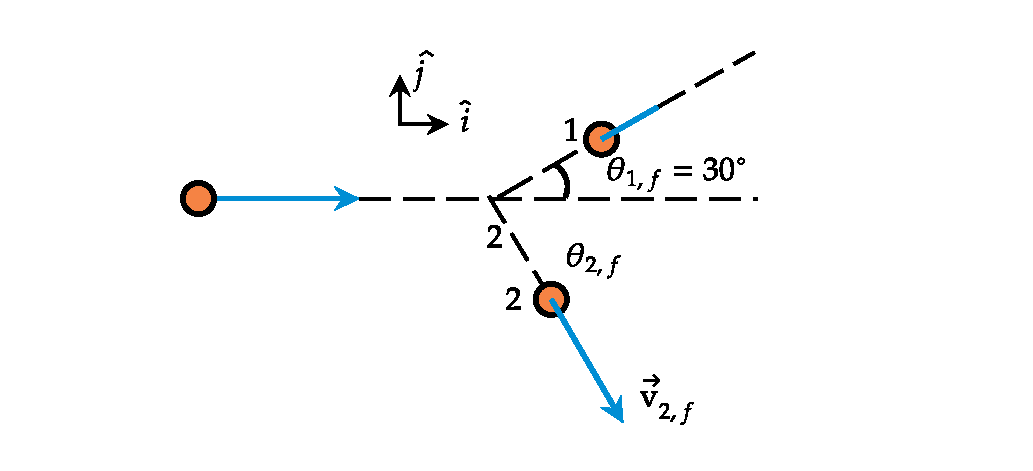
\includegraphics[height=5cm,width=8cm]{diagram-20220218(2)}
	\end{figure}
\end{exercise}
\begin{answer}
 Because the masses are equal, $\alpha=1$. We are given that $v_{1, i}=3.0 \mathrm{~m} \cdot \mathrm{s}^{-1}$ and $\theta_{1, f}=30^{\circ}$. Hence  $0=(1+\alpha) v_{1, f}^{2}-2 \alpha v_{1, i} v_{1, f} \cos \theta_{1, f}-(1-\alpha) v_{1, i}^{2}$ reduces  to
$$ v_{1, f}=v_{1, i} \cos \theta_{1, f}=\left(3.0 \mathrm{~m} \cdot \mathrm{s}^{-1}\right) \cos 30^{\circ}=2.6 \mathrm{~m} \cdot \mathrm{s}^{-1} $$
substitute this value in 
$$\tan \theta_{2, f}=\frac{v_{1, f} \sin \theta_{1, f}}{v_{1, i}-v_{1, f} \cos \theta_{1, f}}$$
$$\begin{aligned}
	\theta_{2, f} &=\tan ^{-1}\left(\frac{v_{1, f} \sin \theta_{1, f}}{v_{1, i}-v_{1, f} \cos \theta_{1, f}}\right) \\
	\theta_{2, f} &=\tan ^{-1}\left(\frac{\left(2.6 \mathrm{~m} \cdot \mathrm{s}^{-1}\right) \sin \left(30^{\circ}\right)}{3.0 \mathrm{~m} \cdot \mathrm{s}^{-1}-\left(2.6 \mathrm{~m} \cdot \mathrm{s}^{-1}\right) \cos \left(30^{\circ}\right)}\right) \\
	&=60^{\circ} .
\end{aligned}$$	
The above results for $v_{1, f}$ and $\theta_{2, f}$ may be substituted into either of the expressions in $m_{2} v_{2, f} \cos \theta_{2, f}=m_{1}\left(v_{1, i}-v_{1, f} \cos \theta_{1, f}\right)$  to find $v_{2, f}=1.5 \mathrm{~m} \cdot \mathrm{s}^{-1}$. 
\end{answer}
\subsection{ Two-Dimensional Collision in Center-of-Mass Reference Frame}
Consider a collision between particle 1 of mass $m_{1}$ and velocity $\overrightarrow{\mathbf{v}}_{1, i}$ and particle 2 of mass $m_{2}$ at rest in the laboratory frame. Particle 1 is scattered elastically through a scattering angle $\Theta$ in the center-of-mass frame. The center-of-mass velocity is given by\\
$$\overrightarrow{\mathbf{v}}_{c m}=\frac{m_{1} \overrightarrow{\mathbf{v}}_{1, i}}{m_{1}+m_{2}}$$
In the center-of-mass frame, the momentum of the system of two particles is zero
$$
\overrightarrow{\mathbf{0}}=m_{1} \overrightarrow{\mathbf{v}}_{1, i}^{\prime}+m_{2} \overrightarrow{\mathbf{v}}_{2, i}^{\prime}=m_{1} \overrightarrow{\mathbf{v}}_{1, f}^{\prime}+m_{2} \overrightarrow{\mathbf{v}}_{2, f}^{\prime}
$$
Therefore
$$
\begin{aligned}
&\overrightarrow{\mathbf{v}}_{1, i}^{\prime}=-\frac{m_{2}}{m_{1}} \overrightarrow{\mathbf{v}}_{2, i}^{\prime} \\
&\overrightarrow{\mathbf{v}}_{1, f}^{\prime}=-\frac{m_{2}}{m_{1}} \overrightarrow{\mathbf{v}}_{2, f}^{\prime}
\end{aligned}
$$
The energy condition in the center-of-mass frame is
$$
\frac{1}{2} m_{1} v_{1, i}^{\prime 2}+\frac{1}{2} m_{2} v_{2, i}^{\prime 2}=\frac{1}{2} m_{1} v_{1, f}^{\prime 2}+\frac{1}{2} m_{2} v_{2, f}^{\prime 2} .
$$
substitute the value of velocities in this equation yields\\
$$v_{1, i}^{\prime}=v_{1, f}^{\prime}$$
(we are only considering magnitudes). Therefore
$$
v_{2, i}^{\prime}=v_{2, f}^{\prime} .
$$
Because the magnitude of the velocity of a particle in the center-of-mass reference frame is proportional to the relative velocity of the two particles, imply that the magnitude of the relative velocity also does not change\\
$$\left|\overrightarrow{\mathbf{V}}_{1,2, i}^{\prime}\right|=\left|\overrightarrow{\mathbf{V}}_{1,2, f}^{\prime}\right|$$
 Recall that the relative velocity is independent of the reference frame\\
 $$\overrightarrow{\mathbf{V}}_{1, i}-\overrightarrow{\mathbf{V}}_{2, i}=\overrightarrow{\mathbf{V}}_{1, i}^{\prime}-\overrightarrow{\mathbf{V}}_{2, i}^{\prime}$$
 In the laboratory reference frame $\overrightarrow{\mathbf{v}}_{2, i}=\overrightarrow{\mathbf{0}}$, hence the initial relative velocity is $\overrightarrow{\mathbf{v}}_{1,2, i}^{\prime}=\overrightarrow{\mathbf{v}}_{1,2, i}=\overrightarrow{\mathbf{v}}_{1, i}$, and the velocities in the center-of-mass frame of the particles are then
 $$\begin{gathered}
 \overrightarrow{\mathbf{v}}_{1, i}^{\prime}=\frac{\mu}{m_{1}} \overrightarrow{\mathbf{v}}_{1, i} \\
 \overrightarrow{\mathbf{V}}_{2, i}^{\prime}=-\frac{\mu}{m_{2}} \overrightarrow{\mathbf{v}}_{1, i}
 \end{gathered}$$
 Therefore the magnitudes of the final velocities in the center-of-mass frame are
 $$
 \begin{aligned}
 &v_{1, f}^{\prime}=v_{1, i}^{\prime}=\frac{\mu}{m_{1}} v_{1,2, i}^{\prime}=\frac{\mu}{m_{1}} v_{1,2, i}=\frac{\mu}{m_{1}} v_{1, i} . \\
 &v_{2, f}^{\prime}=v_{2, i}^{\prime}=\frac{\mu}{m_{2}} v_{1,2, i}^{\prime}=\frac{\mu}{m_{2}} v_{1,2, i}=\frac{\mu}{m_{2}} v_{1, i} .
 \end{aligned}
 $$
 \subsection{Relation between scattering angles in laboratory and centre of mass frame for particle undergoing elastic collision}
 Consider a particle of mass $m_1$ moving with velocity $\vec{u_1}$ in the laboratory frame and let it collide with particles of mass $m_2$ at rest ,the collision being perfectly elastic .After collision the incident particle moves with a velocity $\vec{v_1}$ making scattering angle $\theta_{1}$ with the initial direction and the target particle of mass $m_2$ moves with a velocity $\vec{v_2}$ making recoil angle $\theta_{2}$ with the initial direction of motion of $m_1$.The initial path of $m_1$ is along the X- axis and the plane containing $u_1$ and $v_1$ is the X-Y plane as ahown in figure.\\
 \begin{figure}[H]
 	\centering
 	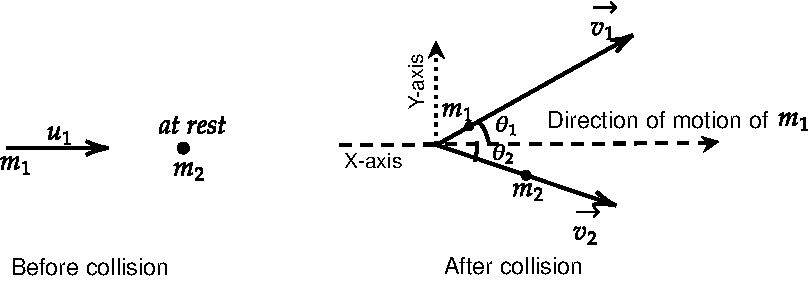
\includegraphics[height=4cm,width=9cm]{diagram-20220221-crop}
 	\caption{}
 	\label{}
 \end{figure}
 Let $\vec{v_1^{\prime}}$ and $\vec{v_2^{\prime}}$ be the final velocities of the particle $m_1$ and $m_2$ after collision in the center of mass frame making an angle $\theta$ with the X-axis as shown in the figure.Then\\
 $\vec{v_1^{\prime}}=\vec{v_1}-\vec{V}_{cm}$ \hspace{1cm} $\vec{v_2^{\prime}}=\vec{v_2}-\vec{V}_{cm}$\\
As $\vec{u_2}=0 ,\quad \vec{V}_{cm}=\frac{m_1u_1}{m_1+m_2}$\\
ie $\vec{V}_{cm}$ and $u_1$ have the same direction along X-axis.Therefore $\vec{V}_{cm}$ has no component along the Y-axis .The y component of the velocity of the particle of mass $m_1$ is the same in both frames.
\begin{equation}
v_1\sin\theta_1=v_1^{\prime}\sin\theta
\end{equation}
As the center of mass has a velocity $\vec{V}_{cm}$ along X-axis with respect to laboratory frame.
\begin{equation}
v_1\cos \theta_{1}=v_1^{\prime}\cos\theta +V_{cm}
\end{equation}
 Divide (1.46) by (1.47),we have \\
 $$\tan\theta_{1}=\frac{v_1^{\prime}\sin\theta}{v_1^{\prime}\cos\theta +V_{cm}}=\frac{\sin\theta}{\cos \theta +\frac{V_{cm}}{v_1^{\prime}}}$$
 But $$V_{\prime}=\frac{m_1}{m_1+m_2}u_1$$
 and $$v_1^{\prime}=\frac{m_2}{m_1+m_2}u_1$$
 Dividing we get $$\frac{V_{cm}}{v_1^{\prime}}=\frac{m_1}{m_2}$$
 $$\tan\theta_1=\frac{\sin\theta}{\cos\theta+\frac{m_1}{m_2}}$$
 Special cases (i)\textbf{when $m_1<<<<m_2$}\\
 in this case $m_1/m_2$ can be neglected and we have 
 $$\tan\theta_{1}=\frac{\sin \theta}{\cos\theta}=\tan\theta$$
 Thus if the incident particle is very light as compared to the target particle ,the angle of scattering for the incident particle in the laboratory and center of mass system are very nearly equal.\\
 Case (ii)\textbf{when $m_1=m_2$}\\
 In this case $m_1/m_2$=1\\
 Hence $$\tan\theta_{1}=\frac{\sin\theta}{1+\cos \theta}=\tan(\theta/2)$$
 $$\theta_{1}=\theta/2$$
 Thus if the incident and target particle are of equal masses ,the angle of scattering in the laboratory system is the half the angle of scattering in the CM system.
 
 
 
 
 
 
 
 
 
 
 
 
 
 
 
 
 
 
 
 
 
 
 
 
 
 
 
 
 
 
 \newpage
 \begin{abox}
 	Practice set 1
 	\end{abox}
 \begin{enumerate}
 	\begin{minipage}{\textwidth}
 	\item The acceleration due to gravity $(g)$ on the surface of Earth is approximately $2.6$ times that on the surface of Mars. Given that the radius of Mars is about one half the radius of Earth, the ratio of the escape velocity on Earth to that on Mars is approximately
 	\exyear{NET JUNE 2011}
 \end{minipage}
 \begin{tasks}(2)
 	\task[\textbf{A.}] $1.1$
 	\task[\textbf{B.}]$1.3$
 	\task[\textbf{C.}]$2.3$
 	\task[\textbf{D.}]$5.2$
 \end{tasks}
\begin{minipage}{\textwidth}
	\item Two particles of identical mass move in circular orbits under a central potential $V(r)=\frac{1}{2} k r^{2}$. Let $l_{1}$ and $l_{2}$ be the angular momenta and $r_{1}, r_{2}$ be the radii of the orbits respectively. If $\frac{l_{1}}{l_{2}}=2$, the value of $\frac{r_{1}}{r_{2}}$ is:
	\exyear{NET DEC 2011}
\end{minipage}
\begin{tasks}(2)
	\task[\textbf{A.}] $\sqrt{2}$
	\task[\textbf{B.}]$1 / \sqrt{2}$
	\task[\textbf{C.}] 2
	\task[\textbf{D.}] $1 / 2$
\end{tasks}
\begin{minipage}{\textwidth}
	\item A planet of mass $m$ moves in the inverse square central force field of the Sun of mass $M$. If the semi-major and semi-minor axes of the orbit are $a$ and $b$, respectively, the total energy of the planet is:
	\exyear{NET DEC 2011}
\end{minipage}
\begin{tasks}(2)
	\task[\textbf{A.}] $-\frac{G M m}{a+b}$
	\task[\textbf{B.}]$-G M m\left(\frac{1}{a}+\frac{1}{b}\right)$
	\task[\textbf{C.}]$-\frac{G M m}{a}\left(\frac{1}{b}-\frac{1}{a}\right)$
	\task[\textbf{D.}]$-G M m\left(\frac{a-b}{(a+b)^{2}}\right)$
\end{tasks}
\begin{minipage}{\textwidth}
	\item A planet of mass $m$ moves in the gravitational field of the Sun (mass $M$ ). If the semimajor and semi-minor axes of the orbit are $a$ and $b$ respectively, the angular momentum of the planet is
	\exyear{NET DEC 2012}
\end{minipage}
\begin{tasks}(2)
	\task[\textbf{A.}]$\sqrt{2 G M m^{2}(a+b)}$
	\task[\textbf{B.}]$\sqrt{2 G M m^{2}(a-b)}$
	\task[\textbf{C.}]$\sqrt{\frac{2 G M m^{2} a b}{a-b}}$
	\task[\textbf{D.}]$\sqrt{\frac{2 G M m^{2} a b}{a+b}}$
\end{tasks}
\begin{minipage}{\textwidth}
	\item A planet of mass $m$ and an angular momentum $L$ moves in a circular orbit in a potential, $V(r)=-k / r$, where $k$ is a constant. If it is slightly perturbed radially, the angular frequency of radial oscillations is
	\exyear{NET JUNE 2013}
\end{minipage}
\begin{tasks}(2)
	\task[\textbf{A.}] $m k^{2} / \sqrt{2} L^{3}$
	\task[\textbf{B.}]$m k^{2} / L^{3}$
	\task[\textbf{C.}]$\sqrt{2} m k^{2} / L^{3}$
	\task[\textbf{D.}]$\sqrt{3} m k^{2} / L^{3}$
\end{tasks}
\begin{minipage}{\textwidth}
	\item The radius of Earth is approximately $6400 \mathrm{~km}$. The height $h$ at which the acceleration due to Earth's gravity differs from $g$ at the Earth's surface by approximately $1 \%$ is
	\exyear{NET DEC 2014}
\end{minipage}
\begin{tasks}(2)
	\task[\textbf{A.}] $64 \mathrm{~km}$
	\task[\textbf{B.}] $48 \mathrm{~km}$
	\task[\textbf{C.}]$32 \mathrm{~km}$
	\task[\textbf{D.}]$16 \mathrm{~km}$
\end{tasks}
\begin{minipage}{\textwidth}
	\item The probe Mangalyaan was sent recently to explore the planet Mars. The inter-planetary part of the trajectory is approximately a half-ellipse with the Earth (at the time of launch),Sun and Mars (at the time the probe reaches the destination) forming the major axis. Assuming that the orbits of Earth and Mars are approximately circular with radii $R_{E}$ and $R_{M}$, respectively, the velocity (with respect to the Sun) of the probe during its voyage when it is at a distance
	\begin{figure}[H]
		\centering
		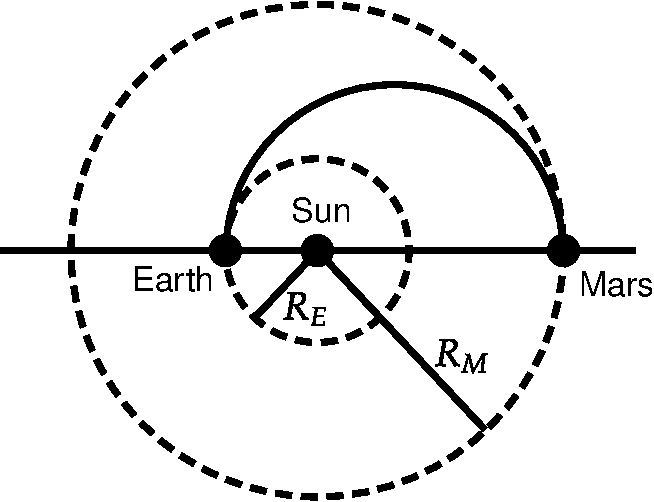
\includegraphics[height=3cm,width=5cm]{diagram-20210926(22)-crop(1)}
	\end{figure}
	$r\left(R_{E}<<r<<R_{M}\right) \text { from the Sun, neglecting the effect of Earth and Mars, is }$
	\exyear{NET DEC 2014}
\end{minipage}
\begin{tasks}(2)
	\task[\textbf{A.}] $\sqrt{2 G M \frac{\left(R_{E}+R_{M}\right)}{r\left(R_{E}+R_{M}-r\right)}}$
	\task[\textbf{B.}]$\sqrt{2 G M \frac{\left(R_{E}+R_{M}-r\right)}{r\left(R_{E}+R_{M}\right)}}$
	\task[\textbf{C.}]$\sqrt{2 G M \frac{R_{E}}{r R_{M}}}$
	\task[\textbf{D.}]$\sqrt{\frac{2 G M}{r}}$
\end{tasks}
\begin{minipage}{\textwidth}
	\item After a perfectly elastic collision of two identical balls, one of which was initially at rest, the velocities of both the balls are non zero. The angle $\theta$ between the final, velocities (in the lab frame) is
	\exyear{NET DEC 2016}
\end{minipage}
\begin{tasks}(2)
	\task[\textbf{A.}] $\theta=\frac{\pi}{2}$
	\task[\textbf{B.}]$\theta=\pi$
	\task[\textbf{C.}]$0<\theta \leq \frac{\pi}{2}$
	\task[\textbf{D.}] $\frac{\pi}{2}<\theta \leq \pi$
\end{tasks}
\begin{minipage}{\textwidth}
	\item Consider circular orbits in a central force potential $V(r)=-\frac{k}{r^{n}}$, where $k>0$ and $0<n<2$. If the time period of a circular orbit of radius $R$ is $T_{1}$ and that of radius $2 R$ is $T_{2}$, then $\frac{T_{2}}{T_{1}}$
	\exyear{NET DEC 2016}
\end{minipage}
\begin{tasks}(2)
	\task[\textbf{A.}] $2^{\frac{n}{2}}$
	\task[\textbf{B.}]$2^{\frac{2}{3} n}$
	\task[\textbf{C.}]$2^{\frac{n}{2}+1}$
	\task[\textbf{D.}]$2^{n}$
\end{tasks}
\begin{minipage}{\textwidth}
	\item A ball weighing $100 \mathrm{gm}$, released from a height of $5 \mathrm{~m}$, bounces perfectly elastically off a plate. The collision time between the ball and the plate is $0.5 \mathrm{~s}$. The average force on the plate is approximately
	\exyear{NET JUNE 2017}
\end{minipage}
\begin{tasks}(2)
	\task[\textbf{A.}] $3 N$
	\task[\textbf{B.}]$2 N$
	\task[\textbf{C.}]$5 N$
	\task[\textbf{D.}]$4 N$
\end{tasks}
\begin{minipage}{\textwidth}
	\item Which of the following figures best describes the trajectory of a particle moving in a repulsive central potential $V(r)=\frac{a}{r}(a>0$ is a constant)?
	\exyear{NET JUNE 2018}
\end{minipage}
\begin{tasks}(2)
	\task[\textbf{A.}]\begin{figure}[H]
		\centering
		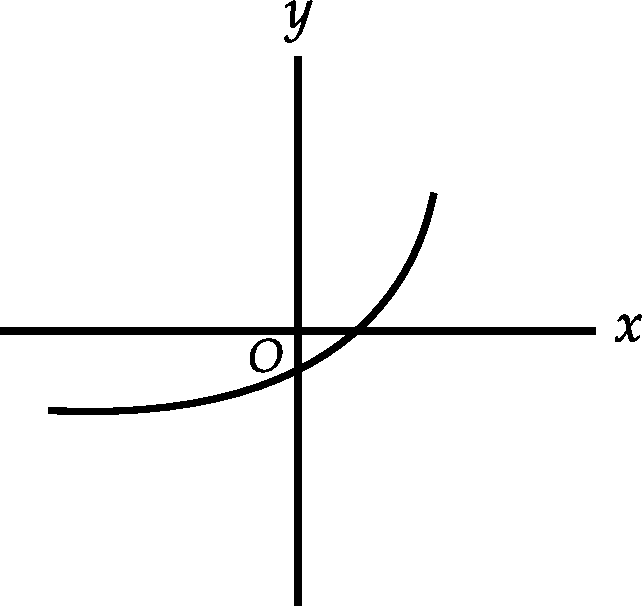
\includegraphics[height=3cm,width=5cm]{diagram-20210926(47)-crop}
	\end{figure}
	\task[\textbf{B.}]\begin{figure}[H]
		\centering
		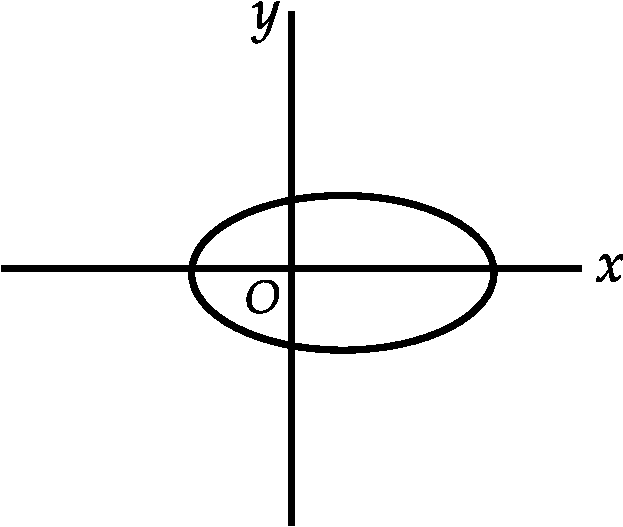
\includegraphics[height=3cm,width=5cm]{diagram-20210926(48)-crop}
	\end{figure}
	\task[\textbf{C.}]\begin{figure}[H]
		\centering
		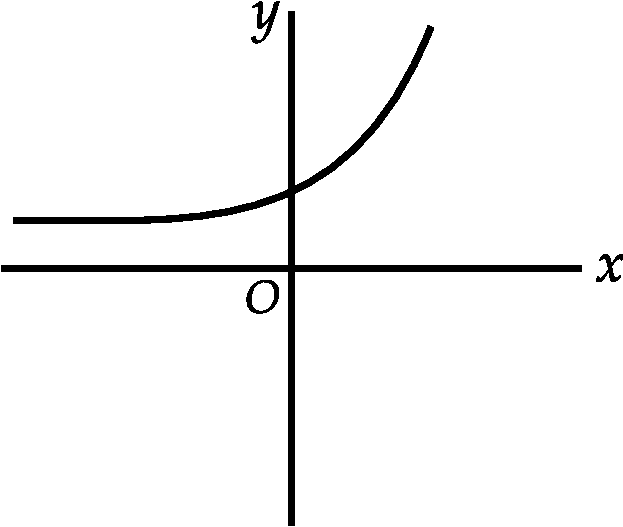
\includegraphics[height=3cm,width=5cm]{diagram-20210926(49)-crop}
	\end{figure}
	\task[\textbf{D.}]\begin{figure}[H]
		\centering
		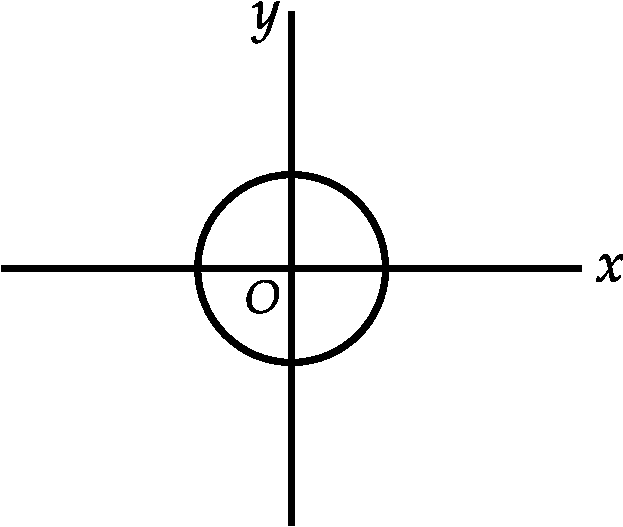
\includegraphics[height=3cm,width=5cm]{diagram-20210926(50)-crop}
	\end{figure}
\end{tasks}
\begin{minipage}{\textwidth}
	\item A particle of mass $m$ moves in a central potential $V(r)=-\frac{k}{r}$ in an elliptic orbit $r(\theta)=\frac{a\left(1-e^{2}\right)}{1+e \cos \theta}$, where $0 \leq \theta<2 \pi$ and $a$ and $e$ denote the semi-major axis and eccentricity, respectively. If its total energy is $E=-\frac{k}{2 a}$, the maximum kinetic energy is
	\exyear{NET JUNE 2018}
\end{minipage}
\begin{tasks}(2)
	\task[\textbf{A.}] $E\left(1-e^{2}\right)$
	\task[\textbf{B.}]$E \frac{(e+1)}{(e-1)}$
	\task[\textbf{C.}]$E /\left(1-e^{2}\right)$
	\task[\textbf{D.}]$E \frac{(e-1)}{(e+1)}$
\end{tasks}
\begin{minipage}{\textwidth}
	\item In the attractive Kepler problem described by the central potential $V(r)=\frac{-k}{r}($ where $k$ is a positive constant), a particle of mass $m$ with a non-zero angular momentum can never reach the centre due to the centrifugal barrier. If we modify the potential to
	$$
	V(r)=-\frac{k}{r}-\frac{\beta}{r^{3}}
	$$
	one finds that there is a critical value of the angular momentum $\ell_{c}$ below which there is no centrifugal barrier. This value of $\ell_{c}$ is
	\exyear{NET DEC 2018}
\end{minipage}
\begin{tasks}(2)
	\task[\textbf{A.}] $\left[12 \mathrm{~km}^{2} \beta\right]^{1 / 2}$
	\task[\textbf{B.}]$\left[12 \mathrm{~km}^{2} \beta\right]^{-1 / 2}$
	\task[\textbf{C.}]$\left[12 \mathrm{~km}^{2} \beta\right]^{1 / 4}$
	\task[\textbf{D.}]$\left[12 \mathrm{~km}^{2} \beta\right]^{-1 / 4}$
\end{tasks}
 \end{enumerate}
\colorlet{ocre1}{ocre!70!}
\colorlet{ocrel}{ocre!30!}
\setlength\arrayrulewidth{1pt}
\begin{table}[H]
	\centering
	\arrayrulecolor{ocre}
	
	\begin{tabular}{|p{1.5cm}|p{1.5cm}||p{1.5cm}|p{1.5cm}|}
		\hline
		\multicolumn{4}{|c|}{\textbf{Answer key}}\\\hline\hline
		\rowcolor{ocrel}Q.No.&Answer&Q.No.&Answer\\\hline
		1&\textbf{c}&2&\textbf{a}\\\hline
		3&\textbf{a}&4&\textbf{d}\\\hline
		5&\textbf{b}&6&\textbf{c}\\\hline
		7&\textbf{b}&8&\textbf{a}\\\hline
		9&\textbf{c}&10&\textbf{d}\\\hline
		11&\textbf{c}&12&\textbf{b}\\\hline
		13&\textbf{c}&&\\\hline
	\end{tabular}
\end{table}